\documentclass{article}
\usepackage[utf8]{inputenc}
\usepackage{amsmath}
\usepackage{listings}
\usepackage{color}
\usepackage{graphicx}
\usepackage[margin=1in]{geometry}
\usepackage{hyperref}
\usepackage{gensymb}
\graphicspath{ {} }

\definecolor{dkgreen}{rgb}{0,0.6,0}
\definecolor{gray}{rgb}{0.5,0.5,0.5}
\definecolor{mauve}{rgb}{0.58,0,0.82}

\lstset{frame=tb,
  language=vhdl,
  aboveskip=3mm,
  belowskip=3mm,
  showstringspaces=false,
  columns=flexible,
  basicstyle={\small\ttfamily},
  numbers=none,
  numberstyle=\tiny\color{gray},
  keywordstyle=\color{blue},
  commentstyle=\color{dkgreen},
  stringstyle=\color{mauve},
  breaklines=true,
  breakatwhitespace=true,
  tabsize=2
}

\title{\textbf{FPGA Temperature Regulation using PID Control \\  University of Connecticut \\ ECE 4401, Final Project}}
\author{David Paquette}
\date{\today}

\begin{document}

\maketitle

\tableofcontents{}
\newpage
\section{Objective}
The objective of this project is to design and build a system to regulate the on board temperature of an FPGA, using PID control in VHDL. The desired temperature must be user selectable during system operation. The desired temperature, current temperature and current fan speed must be displayed on an external display. The current temperature and current fan speed must be collected by an external computer.

\section{Introduction}
\subsection{High Level Overview}
The FPGA development board being used is the Nexys 4 DDR Artix-7. This platform contains a built in temperature sensor and push-button pad, used for reading the onboard FPGA temperature and setting the desired temperature, respectively. To cool the FPGA, a DC computer fan is used, specifically the Asus K52F [4]. To modulate the speed of the fan PWM control is used. Any standard VGA display can be used, the FPGA development board has a standard VGA port built in. The FPGA board can also communicate over UART serial using the built in micro-usb connector, this is used to send fan and temperature data to an external computer. An overview of the components used can be seen in figure 1.
\begin{center}
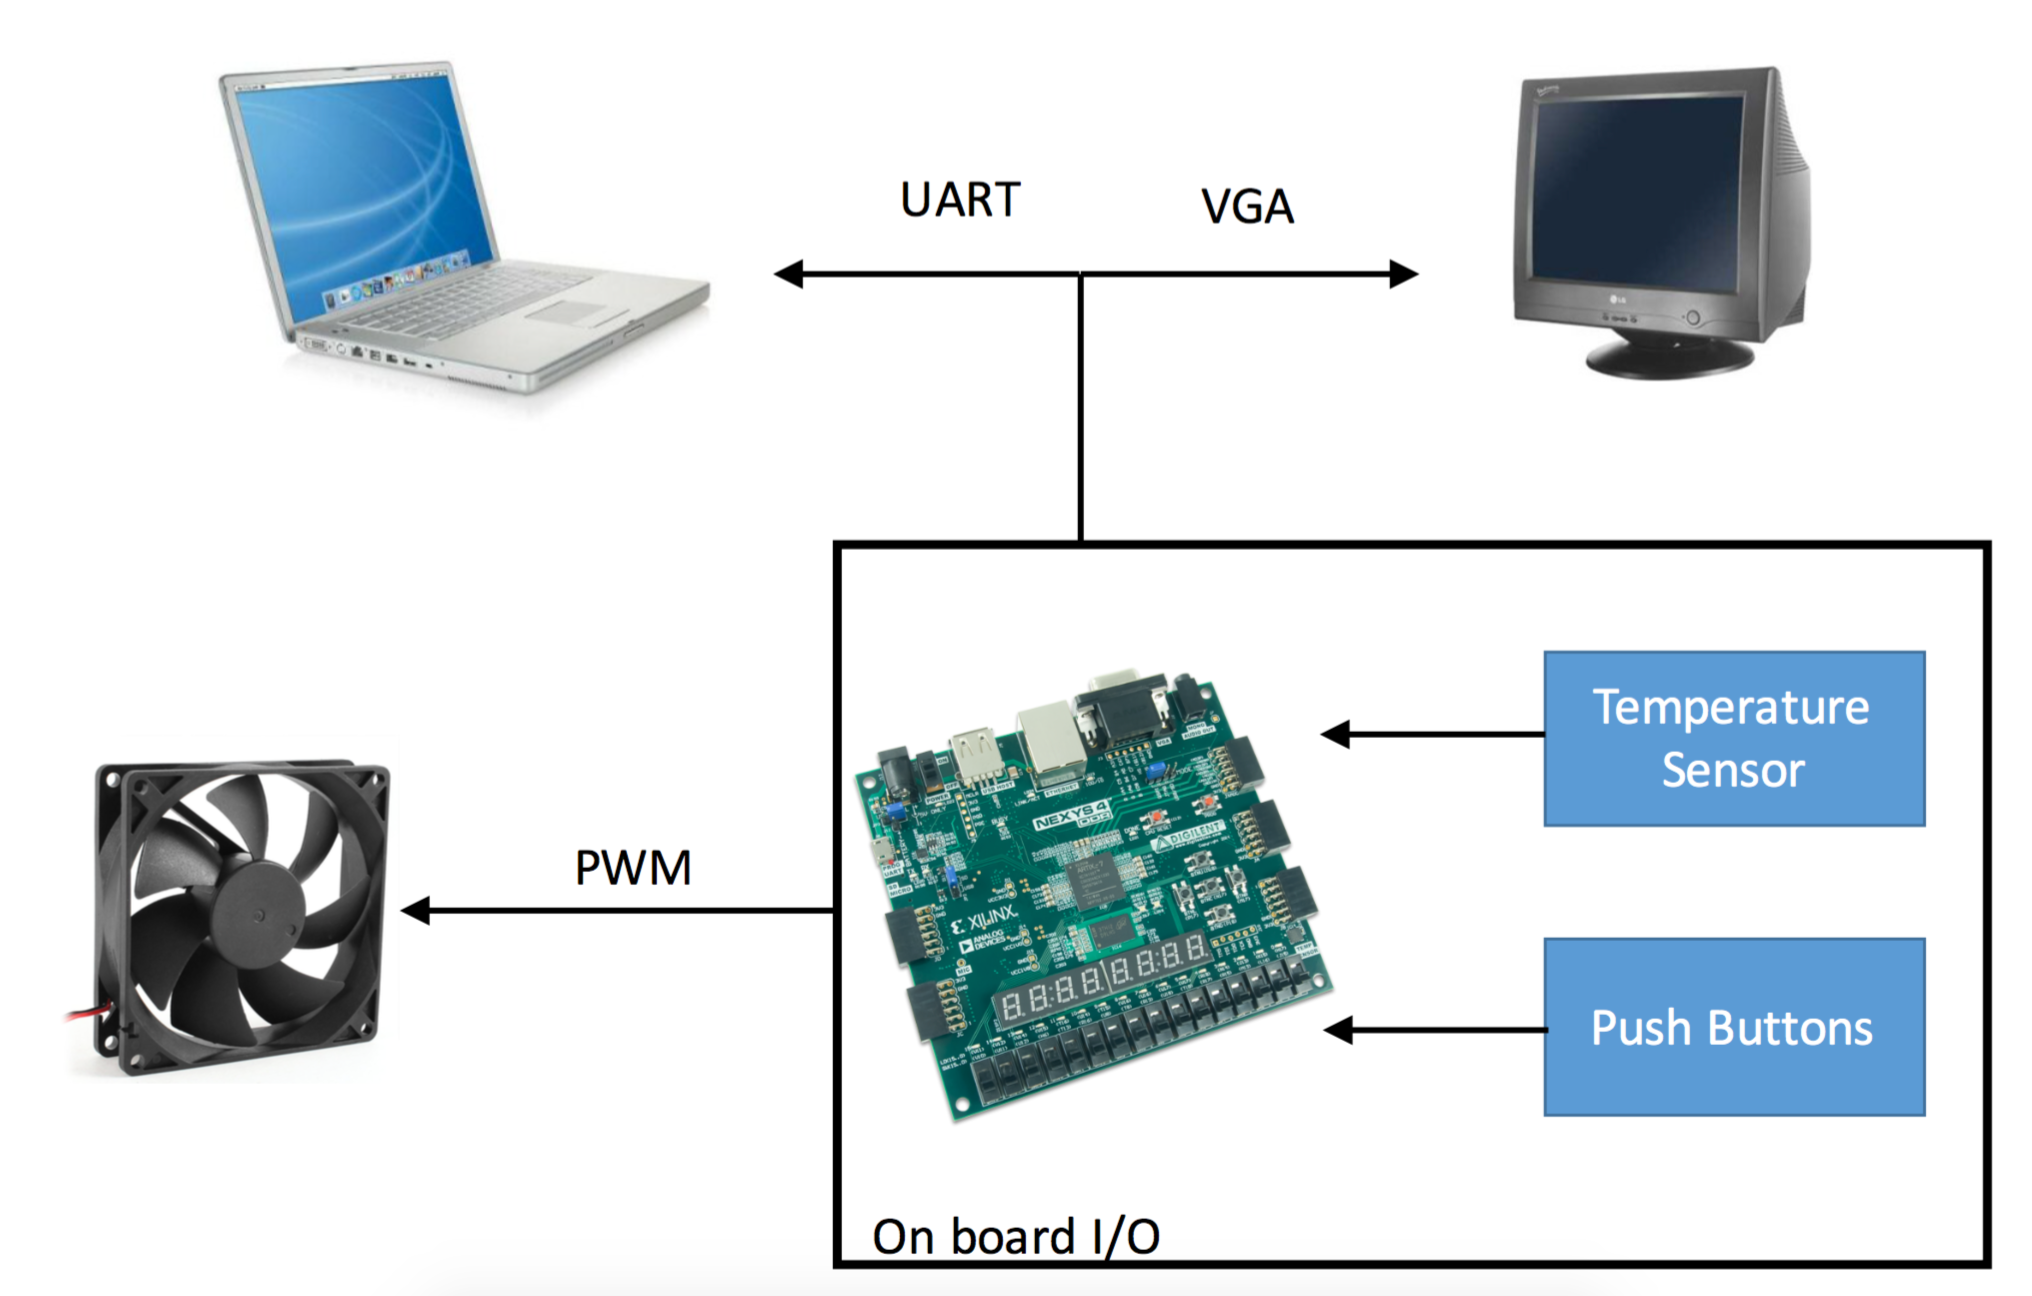
\includegraphics[scale=.4]{images/Overview}\\
\textbf{FIG 1.} High level overview of the system components.\\
\end{center}
\subsection{VHDL Project Overview}
Figure 2 shows an overview of the various VHDL components used in this project. The main modules that were developed for this project were $SetPointControl
$, $PIDController$, $TemperatureSensor$, $PWMInterface$, $Decimal2ASCII$ and $Values2Serial$. The remaining components were originally written for use in other labs but were reused here. The only entity not developed in this course was the $UART$ component. This library was found online in order to speed up the the development of serial data capture, the original source can be seen in [1]. The three highest level components were instantiated in the top level component $TemperatureControlProject$.
\begin{center}
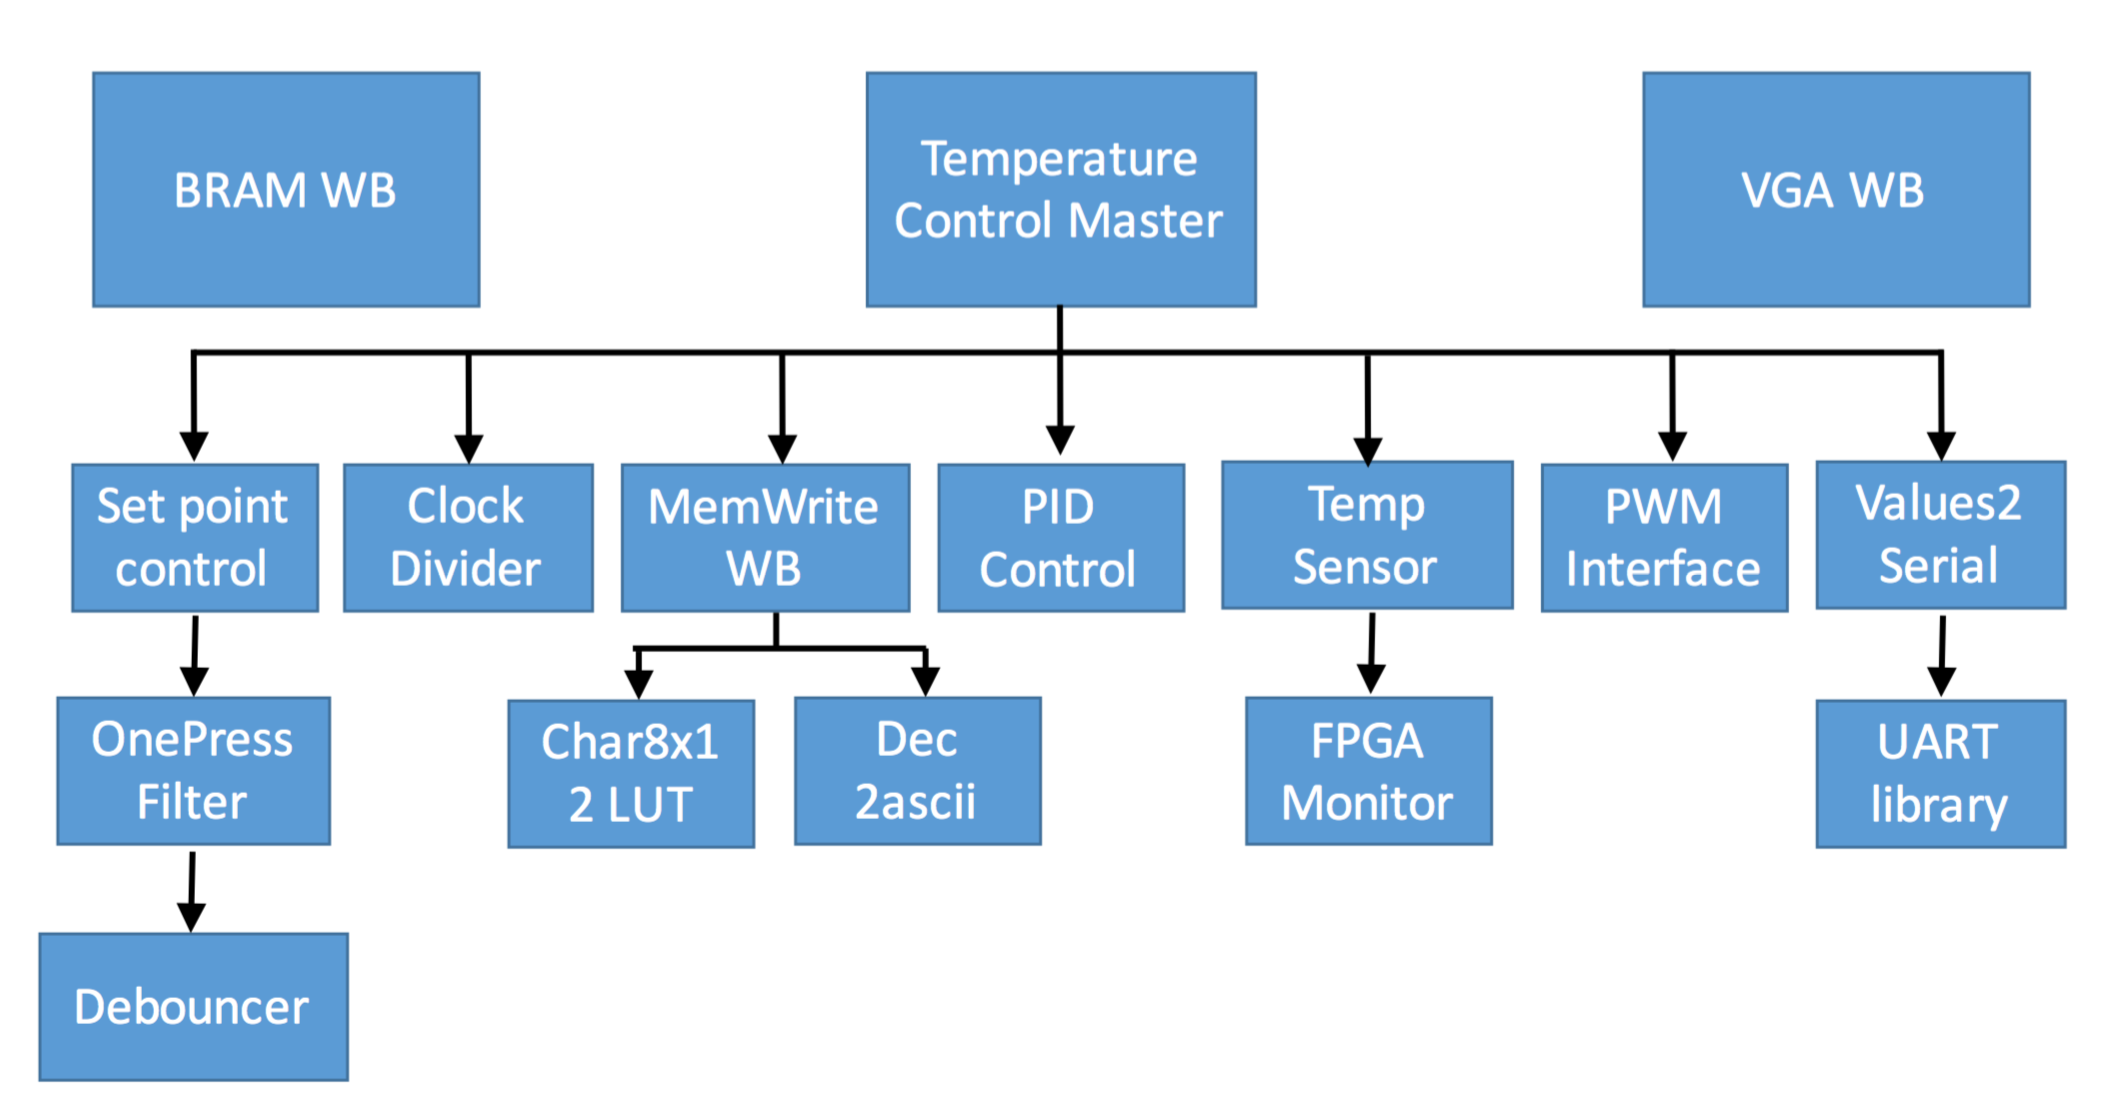
\includegraphics[scale=.35]{images/vhdl_arch}\\
\textbf{FIG 2.} High level VHDL component hierarchy.\\
\end{center}
 
\begin{center}
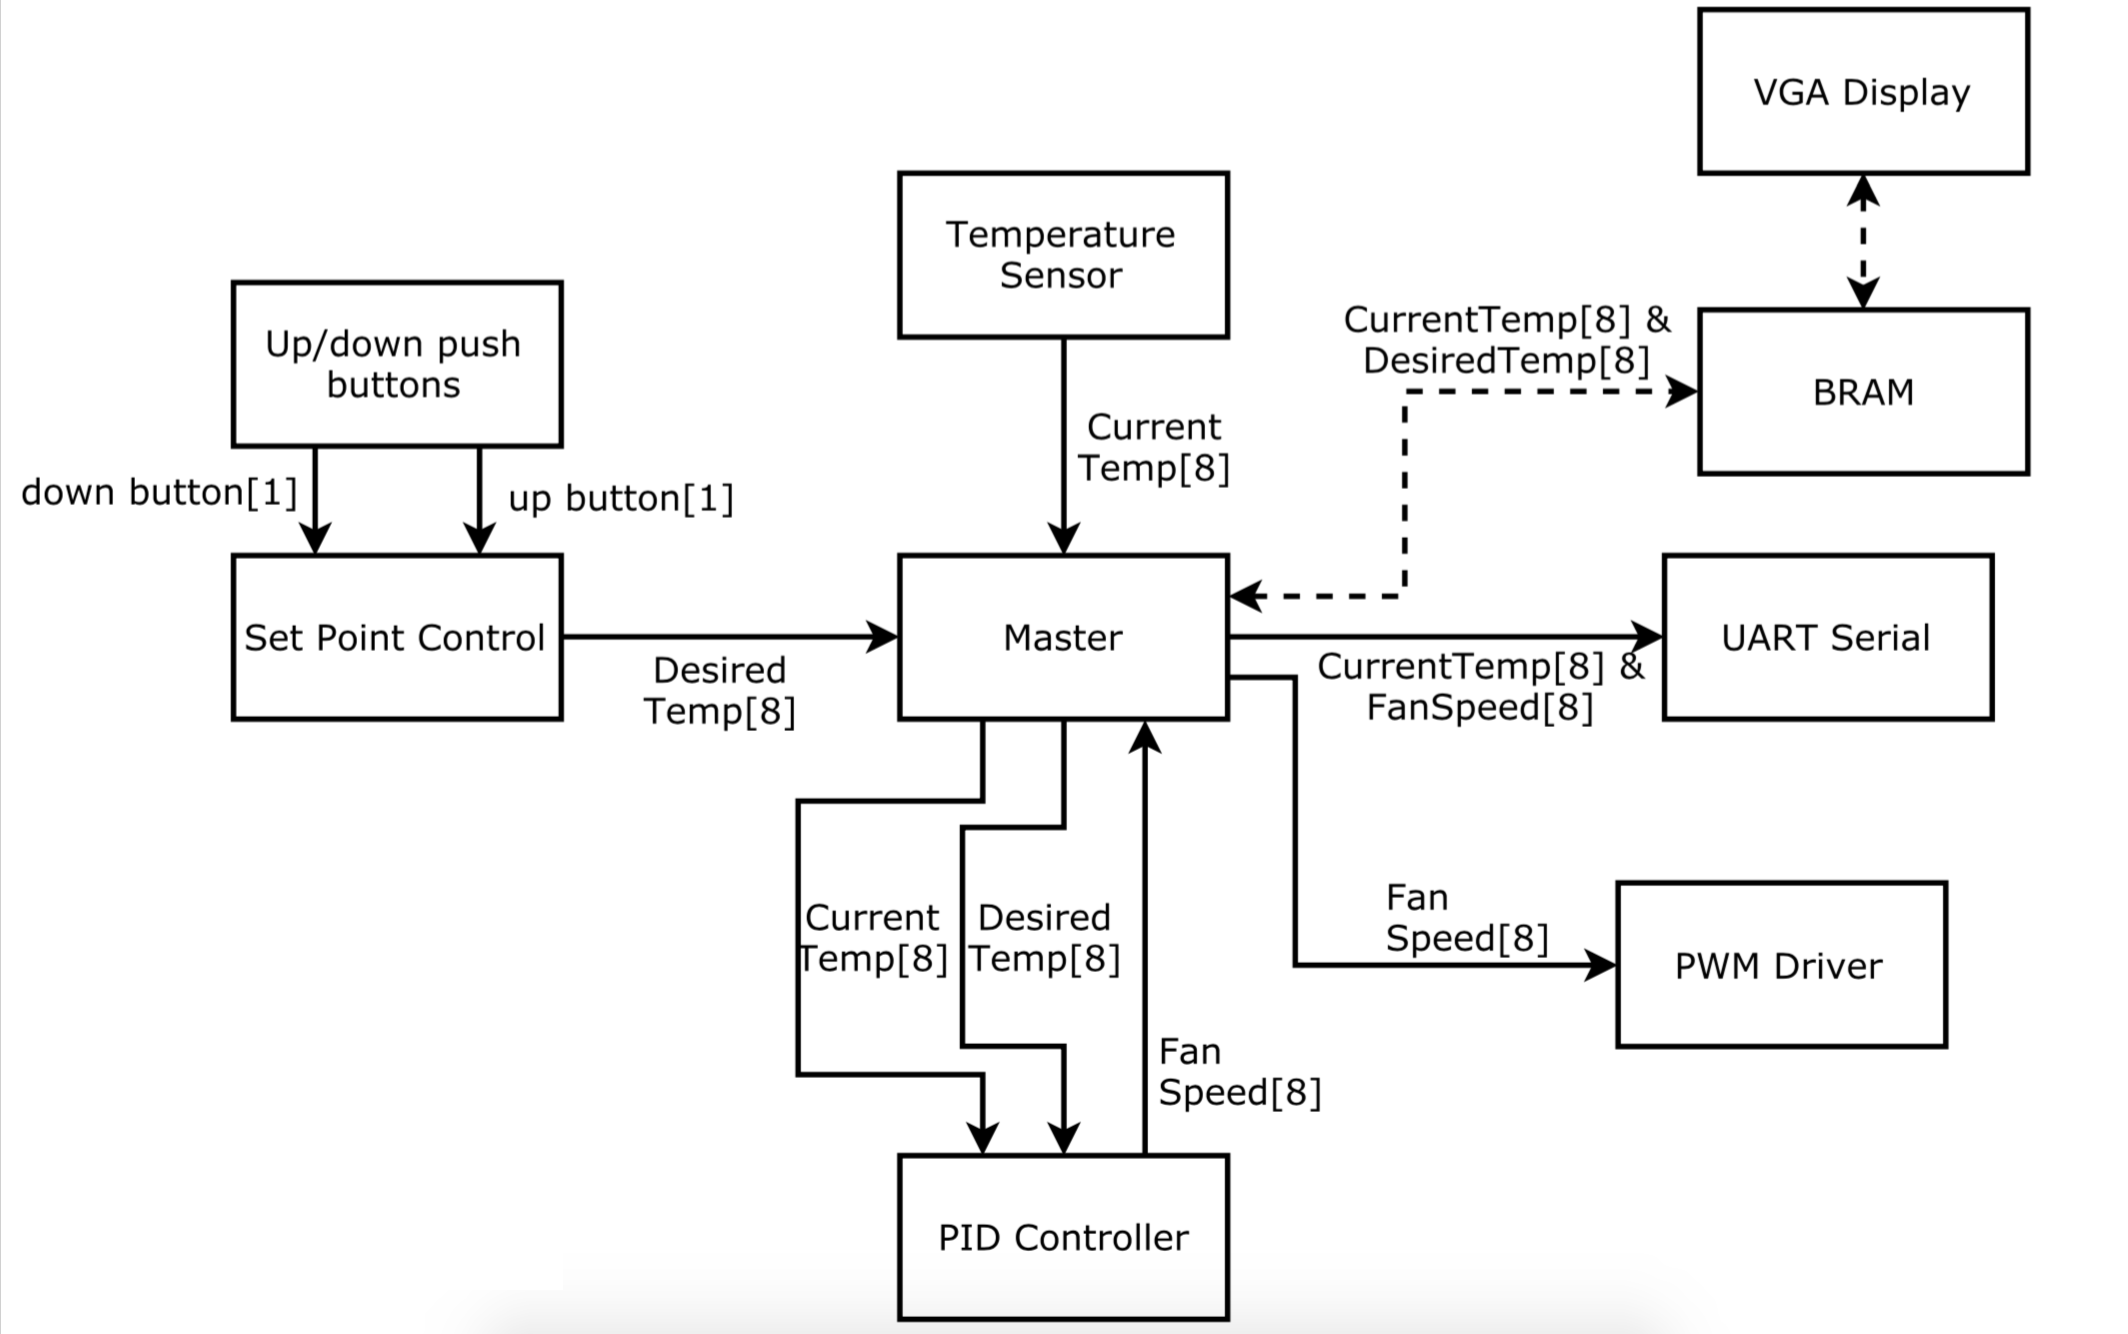
\includegraphics[scale=.4]{images/internalFlow}\\
\textbf{FIG 3.} Main component data path (Wishbone signals are shown as dotted lines).\\
\end{center}

Figure 3 shows the data path of the main components. The $Master$ component contains instantiations of $SetPointControl$, $PIDController$, $PWMDriver$, $TemperatureSensor$ and $UARTSerial$. I decided against making these specific components communicate over the wishbone bus due to the uncertain data send/retrieval time that is introduced when communicating over a central bus. Because digital PID control must be normalized over a constant sampling rate, introducing unknown wait cycles did not seem like a good design choice. It may seem odd that I have the VGA controller communicating over the Wishbone bus but not the UART serial communication. This is because during development I was using the serial connection to collect data for the use of system identification and, once again, I did not want to introduce any unnecessary uncertainties into the data. Because the VGA display is just for the user, and is not a system critical component, any delays introduced by the bus wouldn't be an issue. 

\section{Temperature Sensor Module}
The temperature sensor used was included on the FPGA development board. The sensor is physically located on the FPGA. Xilinx provided documentation on how to read and interpret the data from the sensor [2]. Xilinx also provided a VHDL module, $FPGAMonitor$, for returning the ADC(analog-digital converter) code from the on board temperature sensor. The ADC code then needs to be transformed to a meaningful temperature unit, in this project celsius is used. The equation for transforming the ADC code to a temperature is
\begin{align*}
Temp(\degree C) &= \frac{(ADCode)503.975}{4096}-273.15
\end{align*}
Derived from
\begin{align*}
Voltage &= 10\frac{kT}{q}ln(10)
\end{align*}
Where $k$ is Boltzmann's constant, $T$ is temperature in kelvin and q is the charge on an electron. The analog voltage is sampled by the 12-bit ADCX to produce an ADC code.
 This equation is implemented in the $TemperatureSensorModule$ component. The ADC code is returned in a 12-bit signal, 8-bits for integer values and 4 for decimal. For the sake of simplicity, I will only be using the 8-bits for integer values, which means the accuracy is in $1 \degree$C increments.
\begin{center}
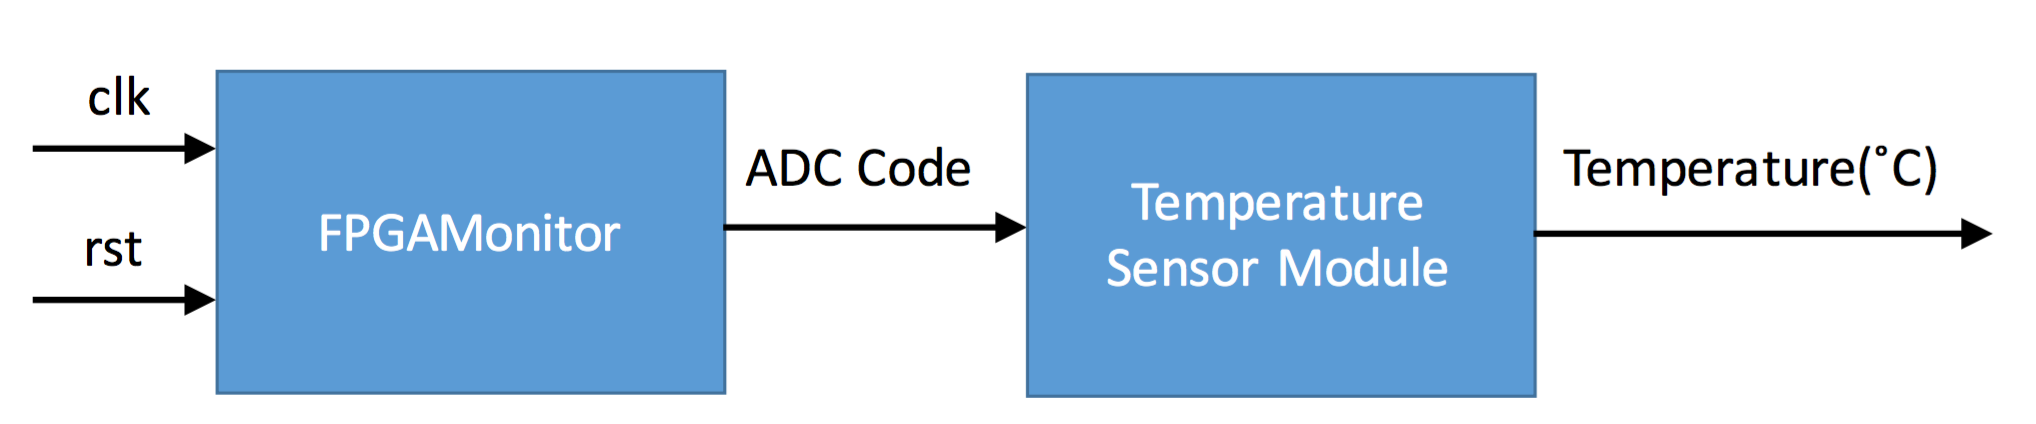
\includegraphics[scale=.4]{images/sensorM}\\
\textbf{FIG 4.} Block diagram of decoding sensor data.\\
\end{center}
\section{Desired Temperature Control Module}
To change the desired temperature during operation two push buttons are used. These buttons are built into the FPGA development board. When pressed, the up button (BTNU) increments the desired temperature and the down button (BTND) decrements the desired temperature. To prevent mechanical glitches and make sure only one change is made per button press, a debouncer and one press filter were used. The state machine for the one press filter can be seen in figure 7. A button press event occurs only in the $press$ state. The $OnePressFilter$ VHDL module contains the button debouncer module. Two instantiations of the $OnePressFilter$ module are made in the $Master$ module. This module outputs a single 8-bit signal, containing the desired temperature.
\begin{center}
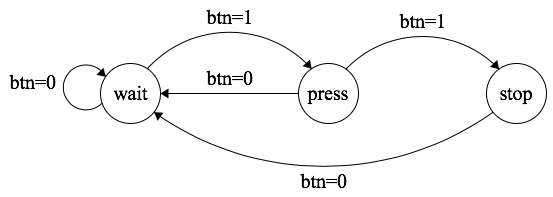
\includegraphics[scale=.5]{images/nopressMachine}\\
\textbf{FIG 5.} State machine diagram of the one press filter.\\
\end{center}
\section{DC Motor Control Module}
To alter the temperature of the FPGA, an off-the-shelf DC computer fan is used [4]. To control the speed of the DC motor the FPGA outputs a PWM signal from the JA PMOD GPIO header. This module takes one 8-bit input signal containing the fan speed, which is limited to an integer with the range of 0 to 100. This value represents the fan speed from 0\% to 100\%. This value is then converted to a duty cycle percent using the logic shown in figure 6.
\begin{center}
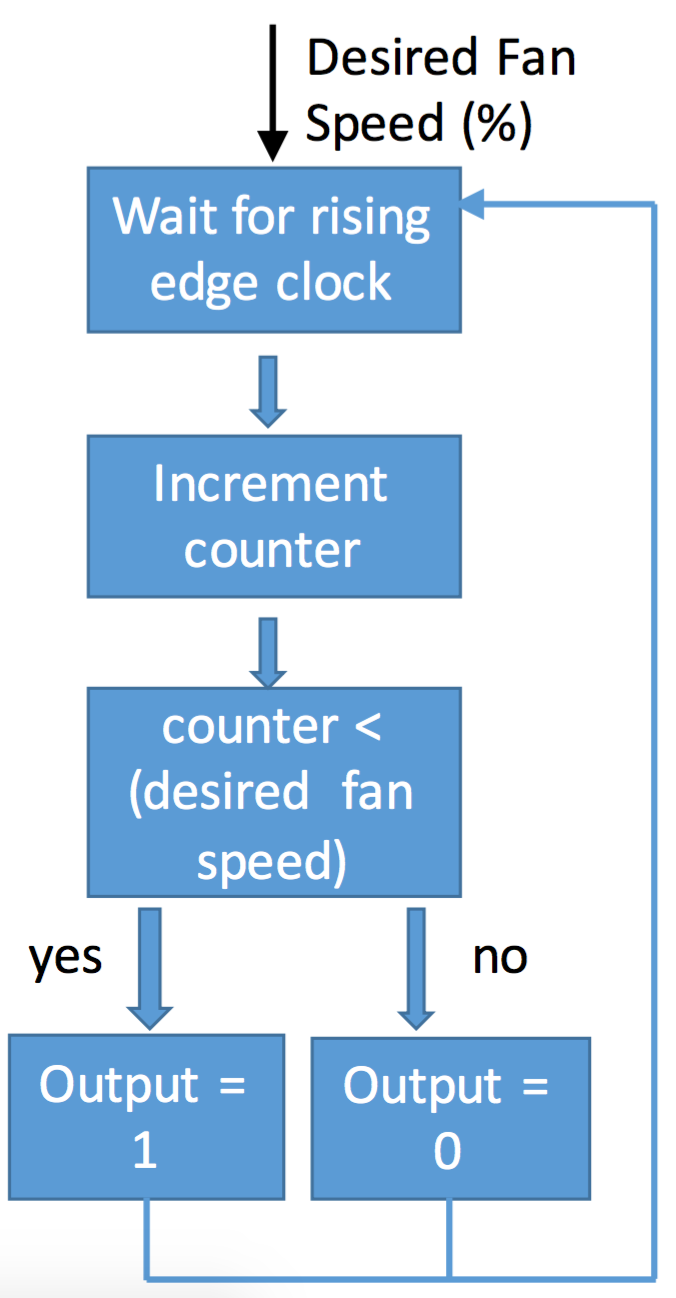
\includegraphics[scale=.4]{images/dutyPWM}\\
\textbf{FIG 6.} Duty cycle(\%) to PWM signal.\\
\end{center}

The FPGA PMOD output is a 0V LOW and 3.3V HIGH signal. However, the DC fan being used requires a potential of 5V. The 3.3V to 5V DC PWM motor driver circuit, shown in figure 7, was used to drive the fan. The circuit uses an n-MOSFET with a low threshold voltage. Specifically, the IRLB721 [3] was used due to its low max threshold voltage ($V_{TH_{max}}=2.35$V). The FPGA was more than adequately able to switch the FET.

\begin{center}
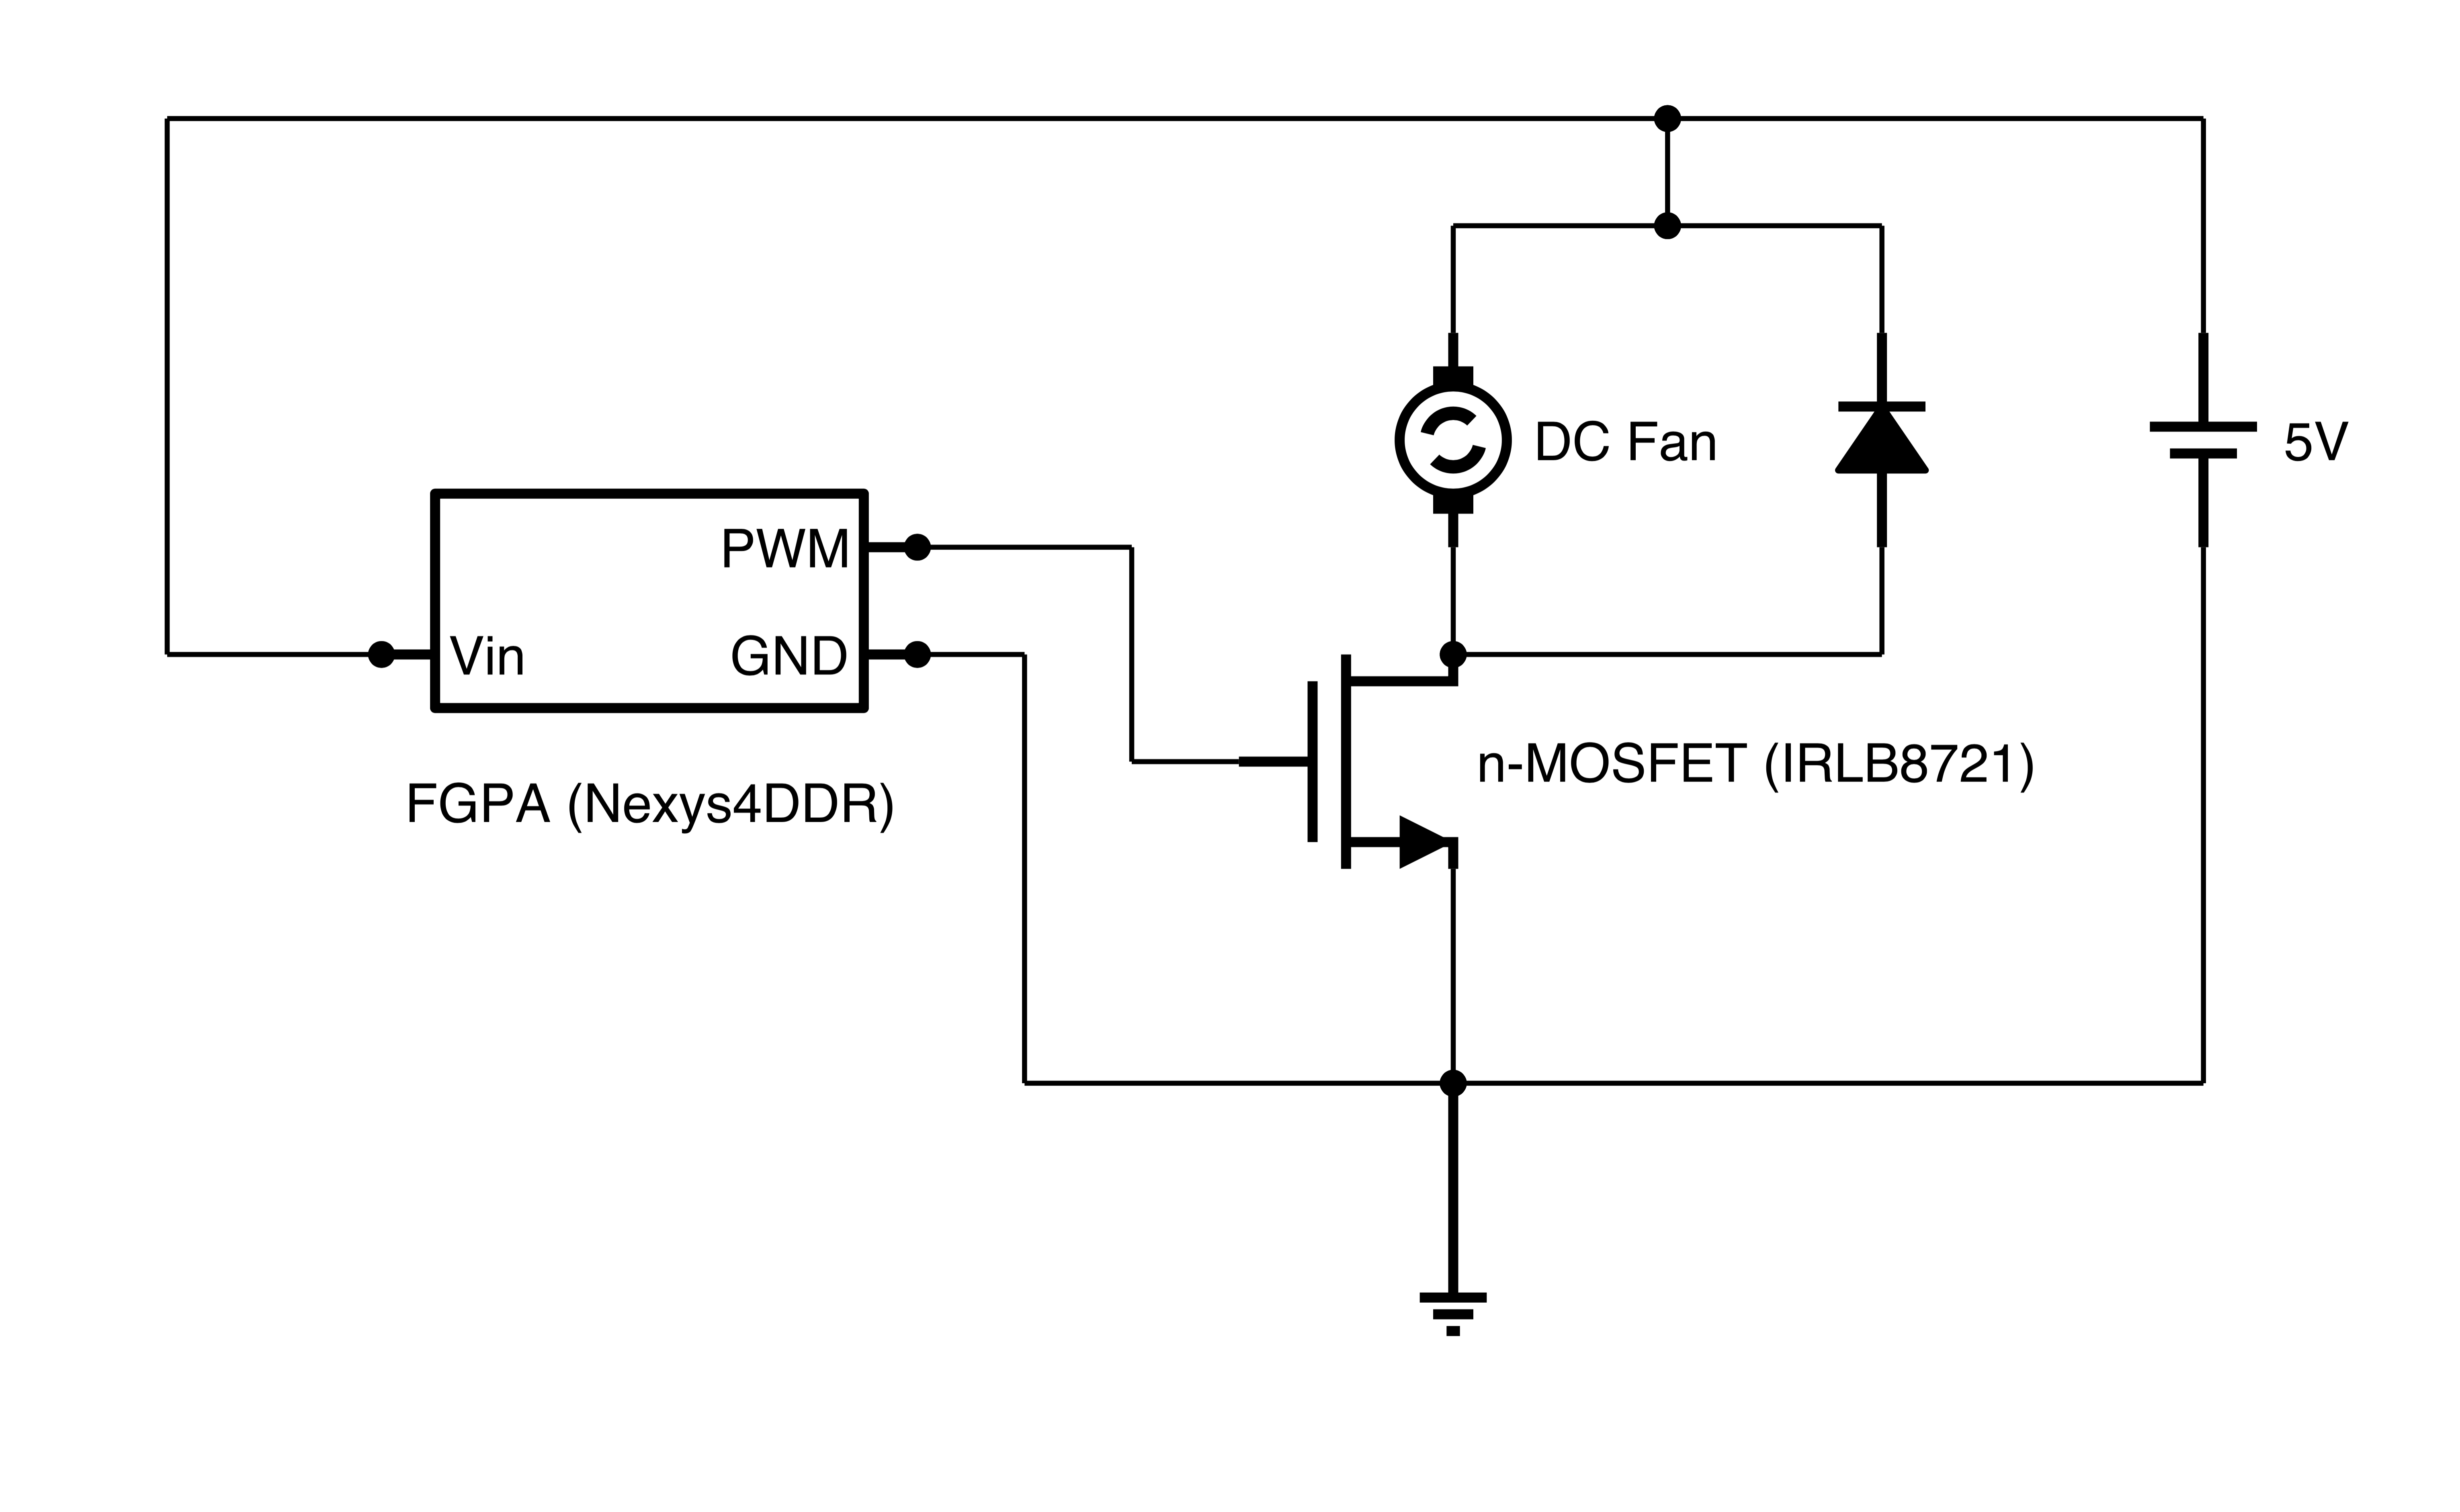
\includegraphics[scale=.5]{images/pwmSchematic-nowords}\\
\textbf{FIG 7.} 3.3V to 5V DC PWM Motor Driver Schematic.\\
\end{center}
\section{UART Serial Communication Module}
\subsection{UART Library Introduction}
For data acquisition I used a UART serial communication between the FPGA and an external computer. However, because this was not the main focus of this project I decided to find a library to simplify UART data transmission. I found a well documented library with plenty of useful examples here [1]. However, to interface with this library another module needed to be created. The $Values2Serial$ module handles interfacing with the UART library. The UART library was contained in a single component and the I/O diagram can be seen in figure 8.
\begin{center} 
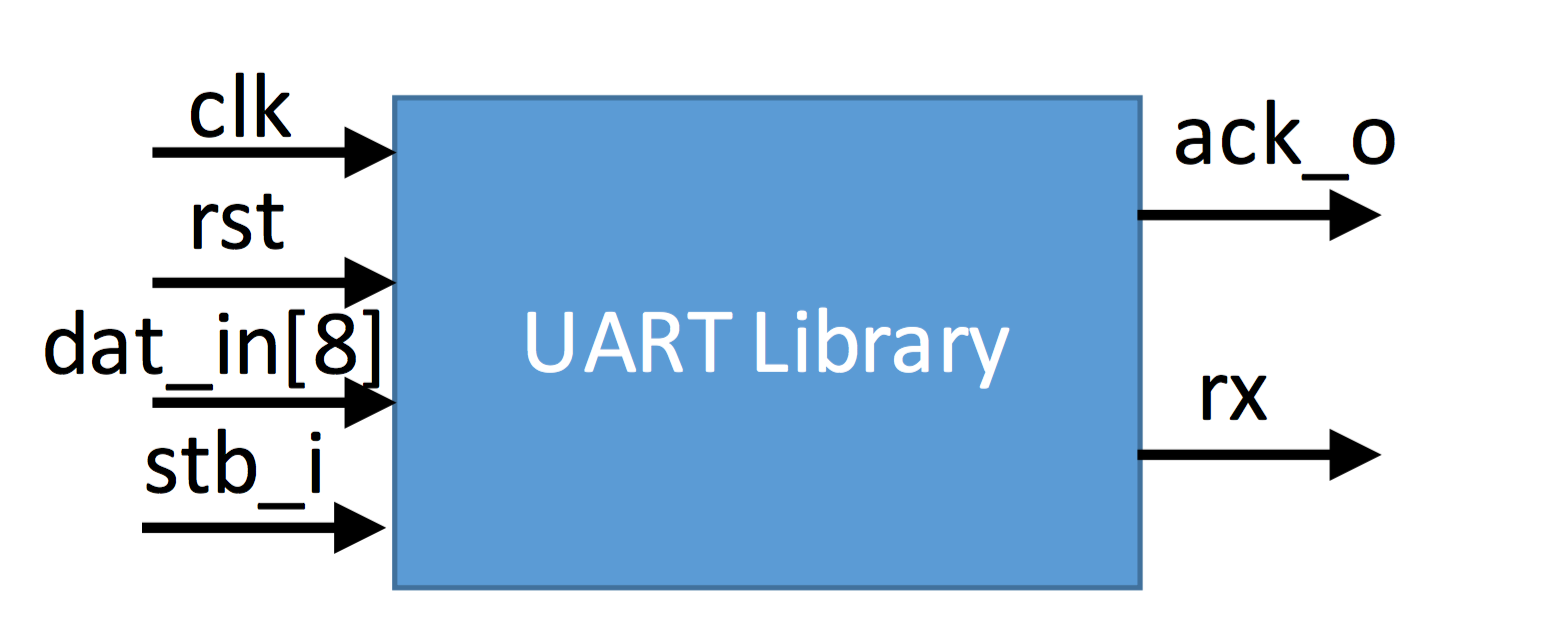
\includegraphics[scale=.35]{images/uartIO}\\
\textbf{FIG 8.} UART library component port map diagram (only relevant ports are shown).\\
\end{center}
Using this library did cause some issues during development. The hardware that the library was developed on used an active high reset scheme, which is opposite from the Nexys 4 DDR, so this caused some minor issues. Another variation was the TX/RX convention used by Xilinx differed from this library. Xilinx uses RX and TX from the perspective of the attached device, in our case this would be the computer. So, the TX port is actually the port where the FPGA receives data and the RX data is the port that the FPGA sends data. This was confusing to work through, but it was well documented in [2].
\begin{center}
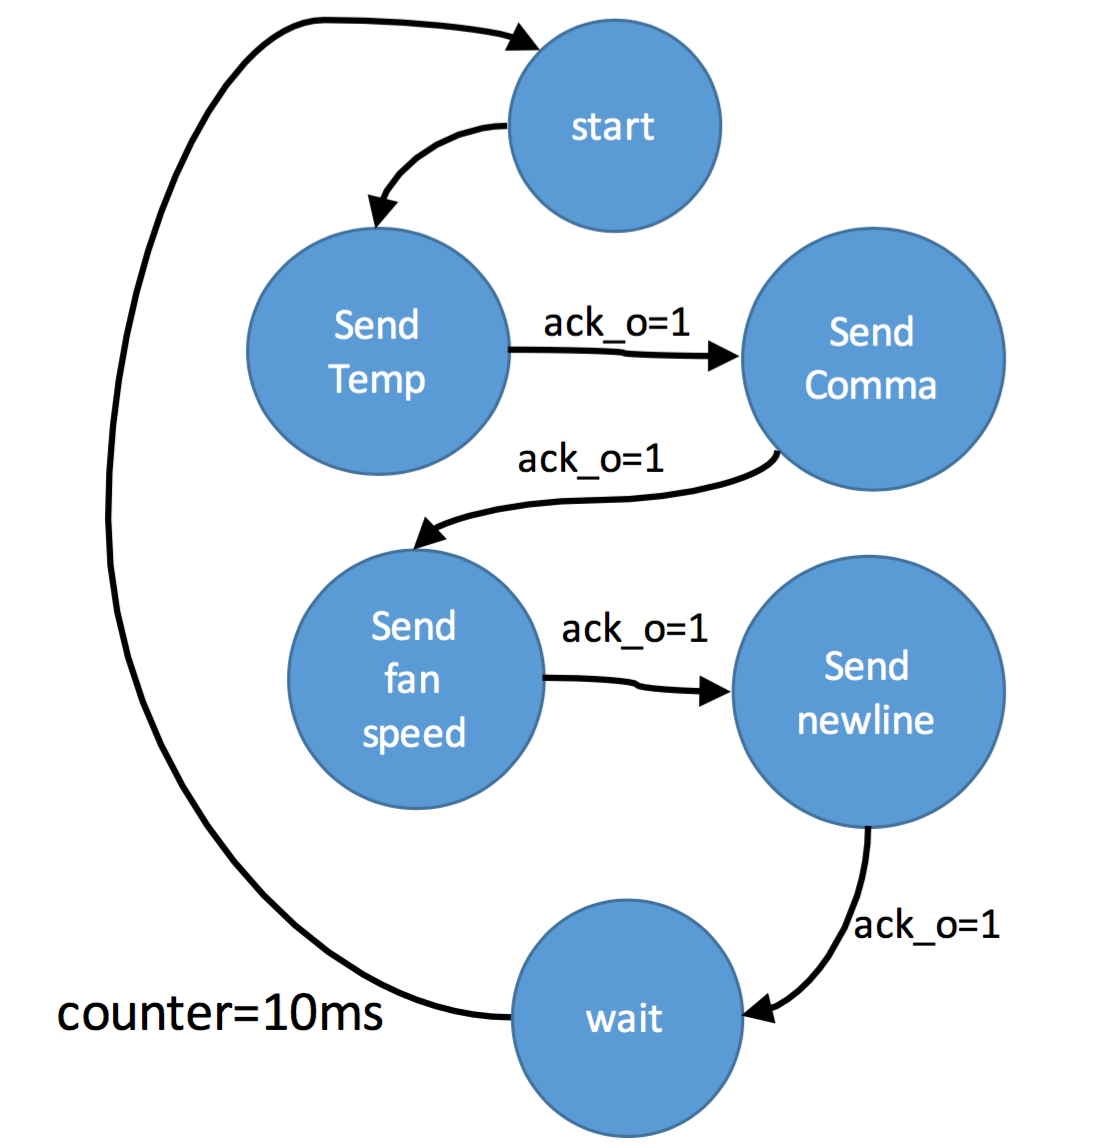
\includegraphics[scale=.35]{images/uartState}\\
\textbf{FIG 9.} State machine for interfacing with the UART library.\\
\end{center}
\subsection{Using the UART Component}
The state machine shown in figure 9 describes how the $Values2Serial$ component interfaces with the UART library. The $UART$ component accepts 8-bit signals, so in order to send a message containing all the required data, a data transmission format was specified. To begin data transfer, the $stb\_i$ pin must be asserted and the data must be placed on the 8-bit $data\_in$ port. We must then wait for the $ack\_o$ to be asserted. When the $ack\_o$ is asserted, we deassert the $stb\_i$ pin and then wait for 10 ms, then repeat the process for the next 8-bit piece of data. 
\subsection{Data Encoding}
	To configure the connection on the external computer any standard serial communication software can be used. However, the settings must be configured to the following settings: baud rate=115200, data bits=8, parity=none, stop bits=1. The data being received will be in the following format: XX2CXX0A. Where the XX represents an 8-bit hexadecimal number, and 2C is the hexadecimal representation of the ASCII comma (,) character and 0A is the hexadecimal representation of the ASCII newline character ($\backslash$n). The first XX contains the current temperature and the second XX contains the current fan speed. Below is an example of the raw serial output. 

\begin{center}
	24 2C 17 0A 24 2C 17 0A 23 2C 17 0A 23 2C 17 0A 22 2C 17 0A 22 2C 17 0A\\
\end{center}
To decode this we start reading it left to right. We first see the hexadecimal 62, if we reference our data format from above, we see that this first number is our current temperature in hexadecimal. For it to be human readable we must convert it to decimal, 0x24 $\rightarrow$ 36. So, the current temperature is $36\degree$C. Moving to the next number we see 2C, again we reference our data format from above and see that this is just ASCII for a comma (,). The next number is hexadecimal 17. Check the format guide and decode to decimal, we can see that this shows the fan speed is 23$\%$. The next number is 0A, which is ASCII for a newline character. This concludes one data reading from the FPGA. Repeat the above procedure to decode the entire message. However, that doesn't seem like very much fun. So, I wrote the below Python script to decode the data for us.

\begin{lstlisting}
f = open('dataFromSerial.txt')
file = open('decodedData.txt', 'w')
data = f.readline().split("0A")
for line in iter(data):
	d = line.split("2C")
	try:
		x = str(int(d[0],16))+ ", " + str(int(d[1],16))
		print(x)
		file.write(x+'\n')
	except ValueError:
		print("there was probably a problem or something")
f.close()
file.close()
\end{lstlisting}
If we pass the above data to this Python function, then we get the following in a much easier to read output format (Current temperature, fan speed).
\begin{center}
36, 23\\
36, 23\\
35, 23\\
35, 23\\
34, 23\\
34, 23\\
\end{center}

\section{VGA BRAM Display Module}
\subsection{VGA Display Overview}
In this project information is first written to the BRAM over the Wishbone bus and is then read from from BRAM over Wishbone by the $VGA$ module. The $VGA$ module was used in previous labs and the implementation won't be discussed here [5]. The module for writing to BRAM was modified from a previous lab. The basics can be seen in figure 10. 
\begin{center}
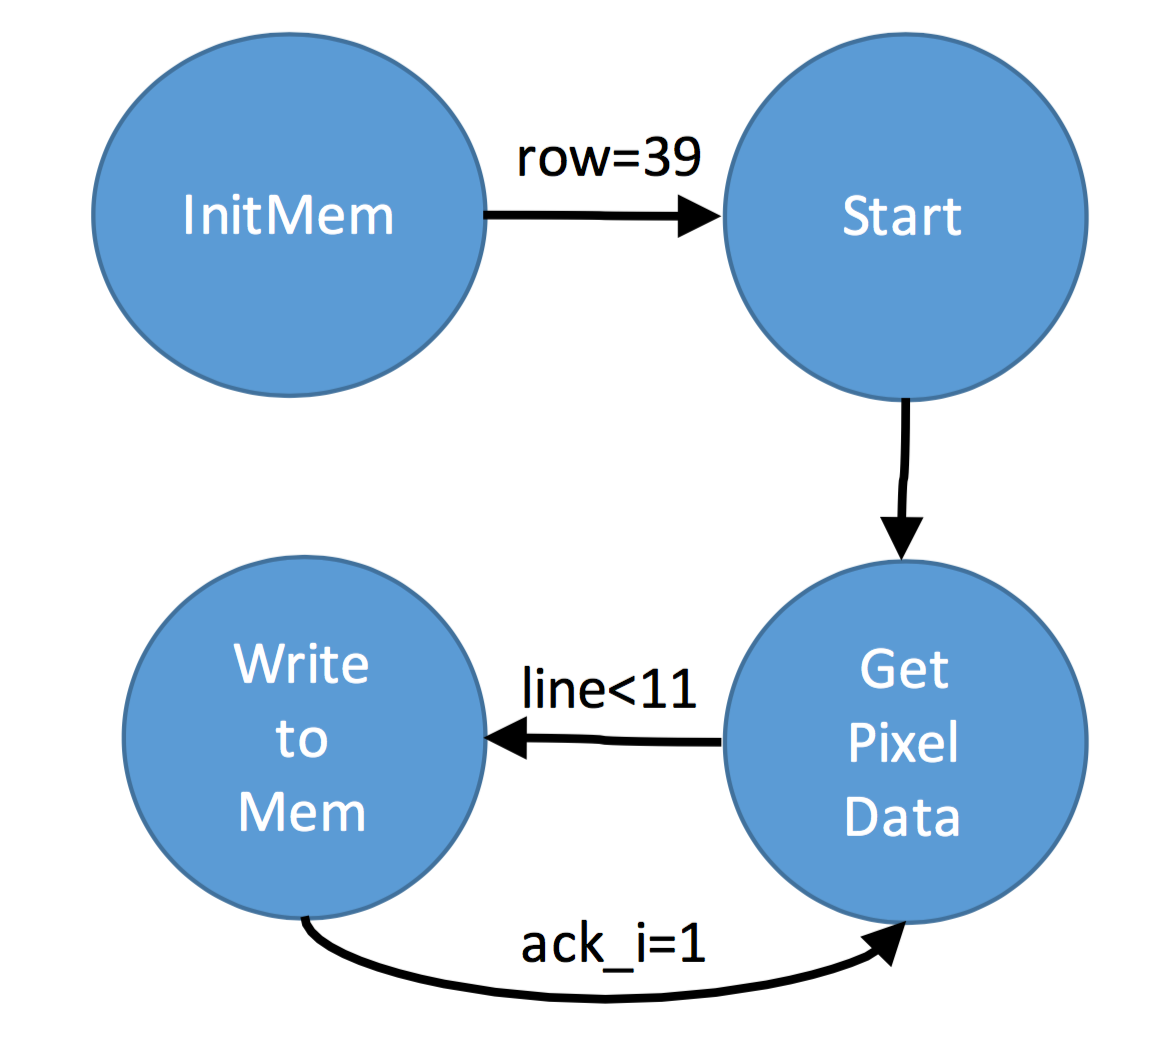
\includegraphics[scale=.35]{images/videoState}\\
\textbf{FIG 10.} State machine for interfacing with the BRAM module over Wishbone.\\
\end{center}
\subsection{BRAM Module}
We start by initializing the BRAM memory by writing all zeros over Wishbone to the BRAM module. The VGA display resolution we used is 640 by 480, and for a single ASCII character we use a block of 11 by 12 giving us a 80 by 40 grid. We first need to convert our hexadecimal ASCII characters to the 11 by 12 pixel map. Once we wait a single clock cycle for the ASCII2Pixel look up table module to complete, we then iterate through the 11 rows and write each one to the BRAM Wishbone bus. The fan speed, current temperature and desired temperature are being displayed on the display. The display format being used is
\begin{align*}
\mathtt{cT}&=\mathtt{XX}\\
\mathtt{dT}&=\mathtt{XX}\\
\mathtt{sF}&=\mathtt{XX}
\end{align*}
Where $\mathtt{cT}$ is the current temperature, $\mathtt{dT}$ is the desired temperature, $\mathtt{sF}$ is the fan speed and the $\mathtt{XX}$ is any decimal integer number from 0 to 99. This means there are 15 characters that need to be written to memory. Each time a character is written the current column is incremented, at the end of the value at each key value pair the row in incremented, at the end of writing the value for the fan speed the row and column is reset to its initial value. One issue I ran into was displaying an integer value 0 to 100 on the display, using the given $ASCII2Pixel$ module. I decided to only display two digits (0 to 99) and if we ever need to display a 100 (most likely for fan speed) the display will show a MV (max value) instead of a number. The method I used to convert a decimal value to its two digit ASCII equivalent is as follows
\begin{align*}
ASCII_{\mathtt{OnesDigit}} &=\mathtt{0x30} + value \bmod 10\\
ASCII_{\mathtt{TensDigit}} &=\mathtt{0x30} + \frac{value-(value\bmod{10})}{10}
\end{align*}
Where $value$ is the integer in range 0 to 100 and $ASCII_{OnesDigit}$ is the ASCII value for the ones place and $ASCII_{TensDigit}$ is the ASCII value for the tens digit. We bias by 0x30 due to standard ASCII convention.
\newpage
\section{Digital PID Control Module}
\subsection{Brief PID Control Theory}
A PID controller is a feedback based controller that modulates an actuator based on the error between desired and current values. Very little information about the system is needed for practical use. PID stands for proportional (P) integral (I) and derivative (D). Each part of the controller has a specific function. The magnitude of influence on the controller output due to each component can be individually tuned. Below is equation for the continuous-time PID controller
\begin{align*}
e(t) &= r(t)-y(t)\\
u(t) &= K_pe(t)+K_i\int e(t)dt + K_d\dfrac{de(t)}{dt}
\end{align*}
Where $e(t)$ is a function of error in terms of time, and is computed by subtracting the reference $r(t)$ by the system output $y(t)$. The reference is also know as the set point or desired value. In our case the reference is the desired temperature, the system output is the current temperature of the FPGA and the input signal $u(t)$ produced by the controller is the fan speed. A block diagram of the system can be seen in figure 11. The $K_p$, $K_i$, and $K_d$ terms are the gains we use to tune each component of the PID controller. Because an FPGA is not a continuous-time system so we need to sample and discretize the above PID equations, these become
\begin{align*}
e[k] &= r[k]-y[k]\\
u[k+1] &= K_pe[k]+K_i\sum e[k]T_s + K_d\dfrac{e[k]-e[k-1]}{T_s}
\end{align*}
Where $T_s$ is our sampling rate, I decided on 10 ms so $Ts=0.01$ seconds.
\begin{center}
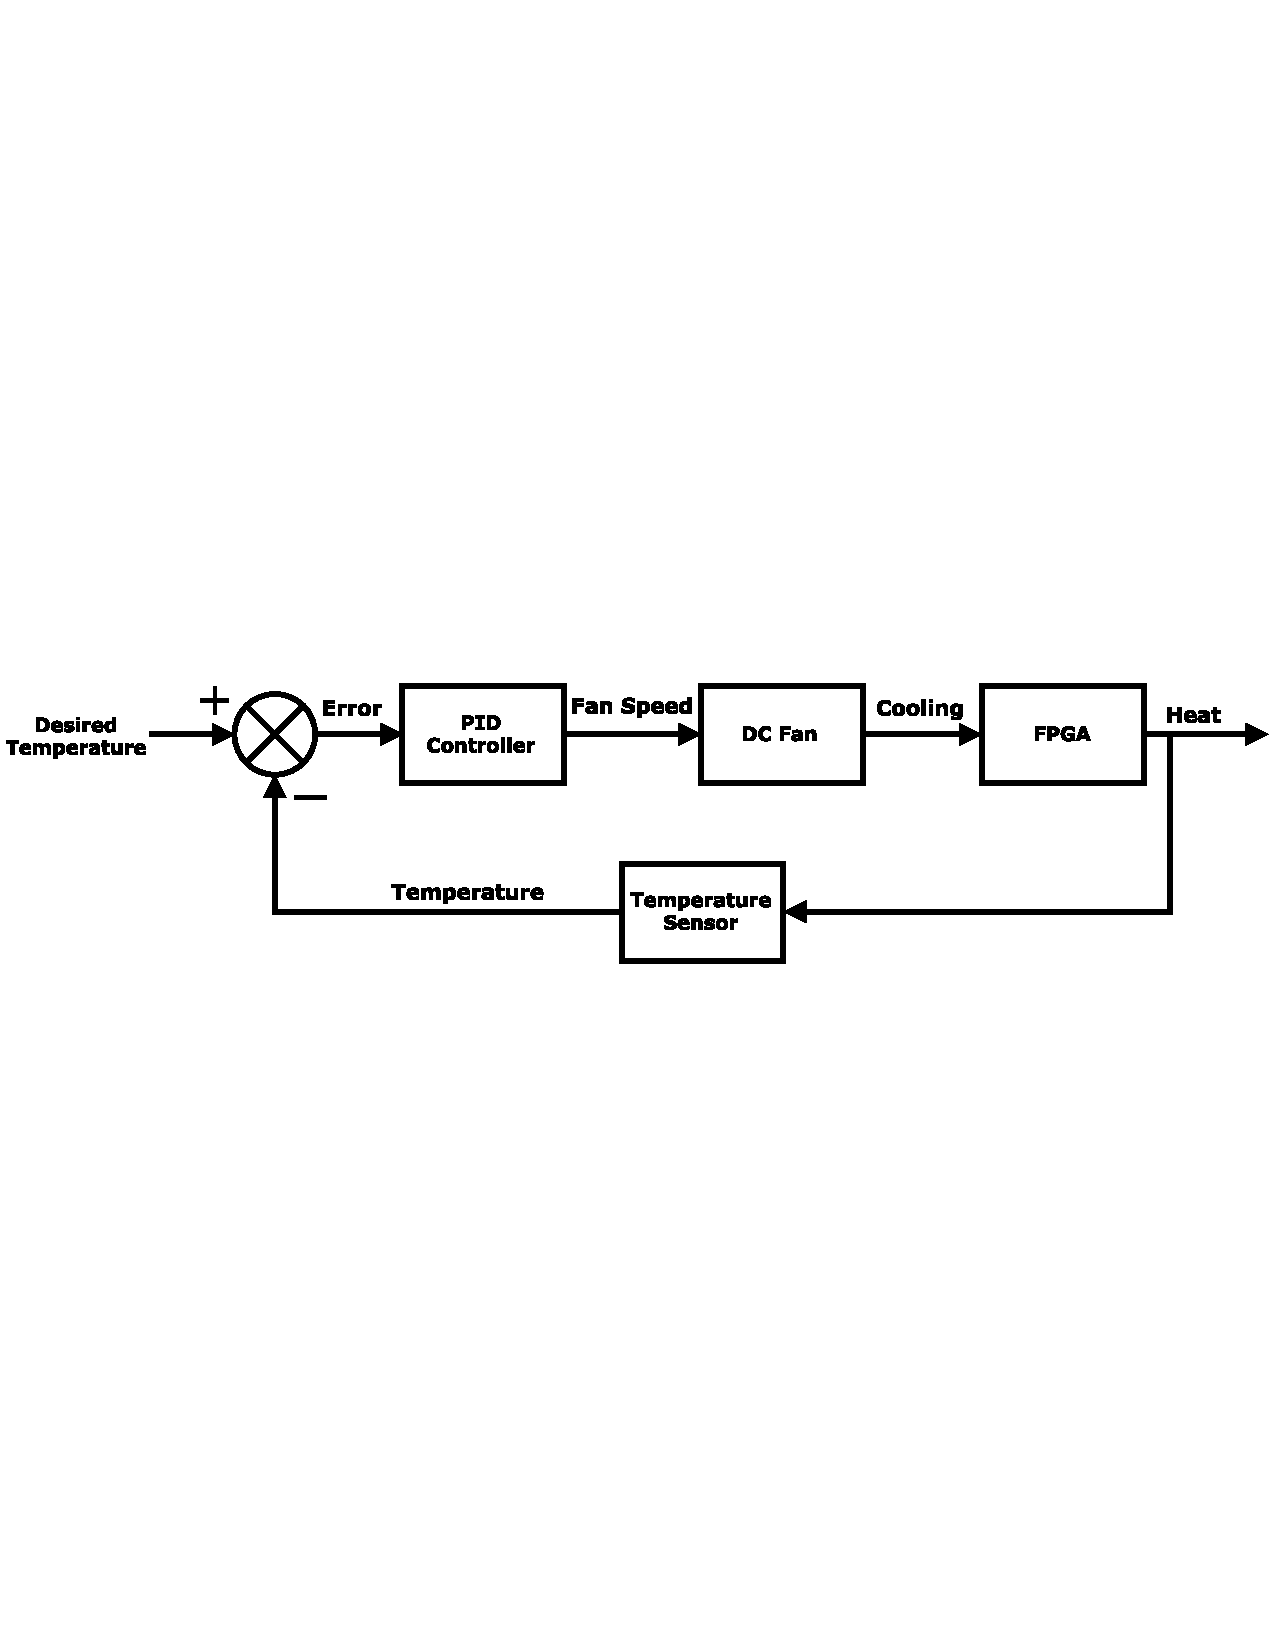
\includegraphics[scale=.75]{images/pidController}\\
\textbf{FIG 11.} Block diagram of FPGA temperature regulation system.\\
\end{center}
\subsection{System Identification}
In order to tune our controller (explained in the following section) a model of our system is a generally useful thing to have. To develop a model we need data that relates the input (fan speed) to the output (FPGA temperature). Using a standard system identification technique, I first set the fan speed to zero. Once the temperature steadied out, I applied a step input of 60\% fan speed to the system. During this process I collected the temperature and fan speed over the UART serial connection, saved it as text file and then used the decoding procedure discussed in section 6.3 to obtain usable data. A plot of the open loop unit step response of the system can be seen in figure 12.
\begin{center}
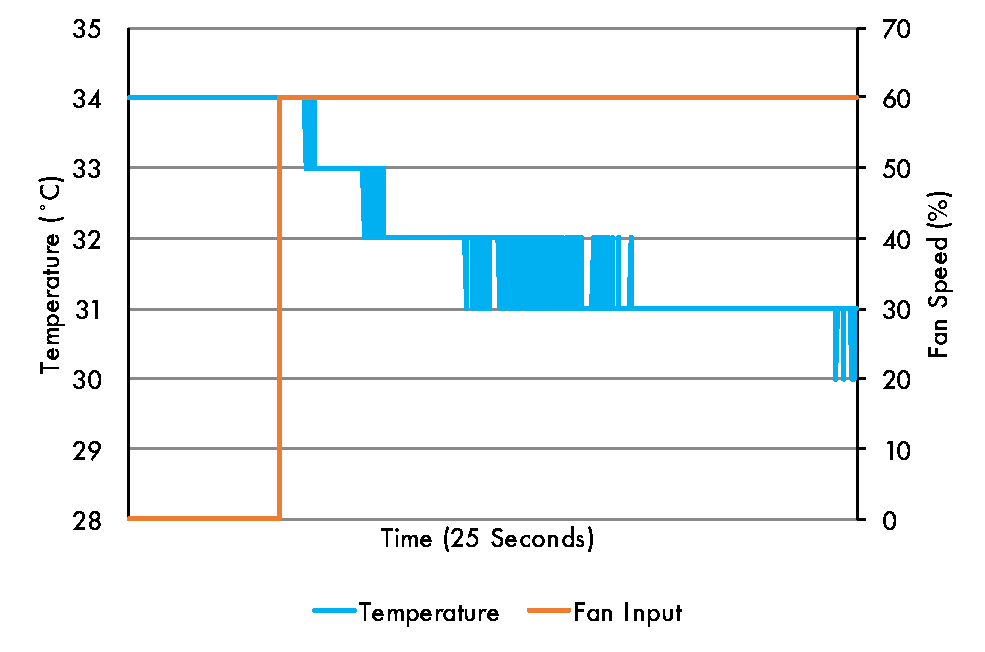
\includegraphics[scale=.75]{images/open_loop}\\
\textbf{FIG 12.} Open loop step response of the system.\\
\end
{center}
As shown in figure 12, as the fan speed is increased to a constant value the temperature exponentially decays to a steady value. I used MATLAB's System Identification toolbox [6] to estimate the input/output relationship between the fan speed and the temperature. However, I had issues using the raw collected data due to the large 1$\degree$C step sizes. So, I first used MATLAB to fit just the output temperature data to a model. The following model was generated
\begin{align*}
m(t) = 3.591e^{-0.0019t}+30.52e^{5.836\times10^{-6}}
\end{align*}
Where $m(t)$ is valid for $t=0$ to $t=2500$, or 0 to 2500 milliseconds.
This model's confidence bound was 95\%. I then used the System Identification toolbox with this model to find the I/O relationship. Because $m(t)$ is a simple exponentially decaying function, I assumed that this it's a first order system. The computed discrete time state-space equation is
\begin{align*}
x[k+1] &= 0.9978x[k]+0.125u[k]\\
y[k] &= -0.08438x[k]
\end{align*}
However, because this is only a single order system, it may be more convenient to represent it using a discrete-time transfer function
\begin{align*}
  G(z)=\frac{-0.01055z^{-1}}{1-0.9978z^{-1}}
\end{align*}
\subsection{Digital PID Controller Design}
The PID gains $K_p$, $K_i$, and $K_d$ gains can be tuned analytically or quantitatively. Analytic tuning typically requires a deep understanding of how the system behaves as well as a good intuition of how each gain affects the transient and steady-state system behavior. This method is more iterative, typically more testing and validation has to occur. Because the system dynamics were estimated in the previous section we can use MATLAB to quantitatively compute our gains, designing for a desired transient and steady-state response. Using MATLAB's PID Tuning [7] toolbox with the system defined above, the below gains were computed
\begin{center}
$K_p=-0.303$	$K_i=-0.123$	$K_d=0$
\end{center}
The first thing that jumps out is that our $K_d$ term is zero. The $K_d$ gain heavily influences rapid changes in the system, because our system is represented by a fairly slowly changing first order differential equation, it is not too much of a surprise that MATLAB computed $K_d$ to equal 0. Something else that stands out is that the other gains are negative. Intuitively this makes sense and was expected. Our actuator's speed is inversely proportional to our process variable. So, an increase in fan speed decreases the FPGA temperature. This physical behavior explains the negative gains.
The below code sample is the VHDL implementation of the discrete-time PID controller shown in section 8.1.
\begin{lstlisting}
elsif(samplingRateClock'event and samplingRateClock='1') then
			error := (setpoint - sensorFeedbackValue); --compute new error e[k]
			errorSum	:= errorSum + error; --continually compute discrete integral
			if(errorSum > 10000) then --integral wind up check
				errorSum := 10000;
			elsif(errorSum < -10000) then
				errorSum := -10000;
			end if;
			errorChange := error - previousError; --compute discrete derivative
			output := (kp*error + ki*errorSum + kd*errorChange)/100; --compute and scale output
			previousError := error; --save error for use in next iteration for discrete derivative
			if(output>100) then --saturate sensor if needed
				output := 100;
			elsif(output<0)then
				output:=0;
			end if;
			controllerOutput<= output;
	end if;
\end{lstlisting}
There are a few differences between a pure PID controller and the above VHDL process. The first is the controller output is being divider by 100. This is due to me avoiding the problem of using decimals (again). I scaled the gains by a factor of 100, so that controller can still compute a full range of output and then it is divided by 100 to scale it back to physically realistic fan speeds. The second difference is the first if/else statement. This prevents the integral term from becoming too large when the controller cannot stabilize the output for whatever reason. If the integral term continually summed up or down to either of its bounds, then the behavior of the system would be undefined and it would act  erratically. The second set of if/else statements is the final defense against the PID controller attempting to set the fan to a value higher than 100\% or less than 0\%.
\begin{center}
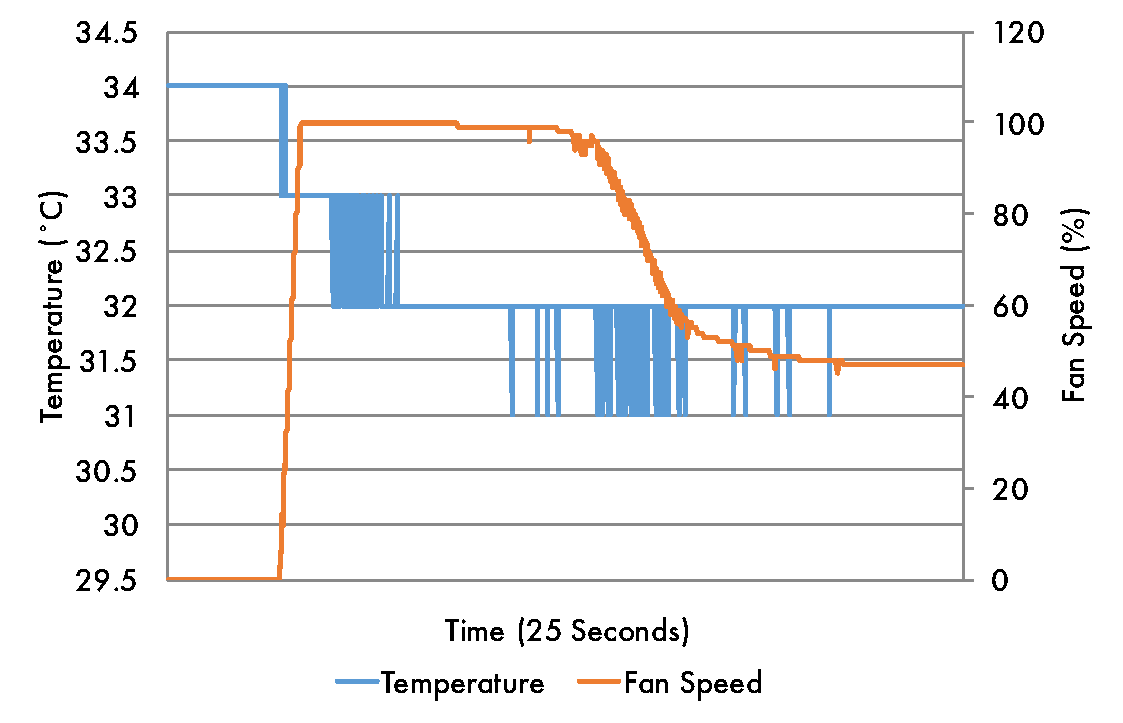
\includegraphics[scale=.75]{images/closed_loop}\\
\textbf{FIG 13.} Closed loop step response of the system, reacting from a set point change of 34$\degree$C to 32$\degree$C.\\
\end
{center}
The PID gains performed well when implemented using the above VHDL process. To test the system, I set the desired temperature to 34$\degree$C and waited for the system to stabilize. I then changed the desired temperature to 32$\degree$C, and collected the data using the serial UART connection. The closed loop system response can be seen in figure 13. There is a small amount of overshoot. After about 20 seconds of settling time, the PID controller's steady state output of 48\% seems to adequately minimize the error.

\section{Implementation Images}
\begin{center}
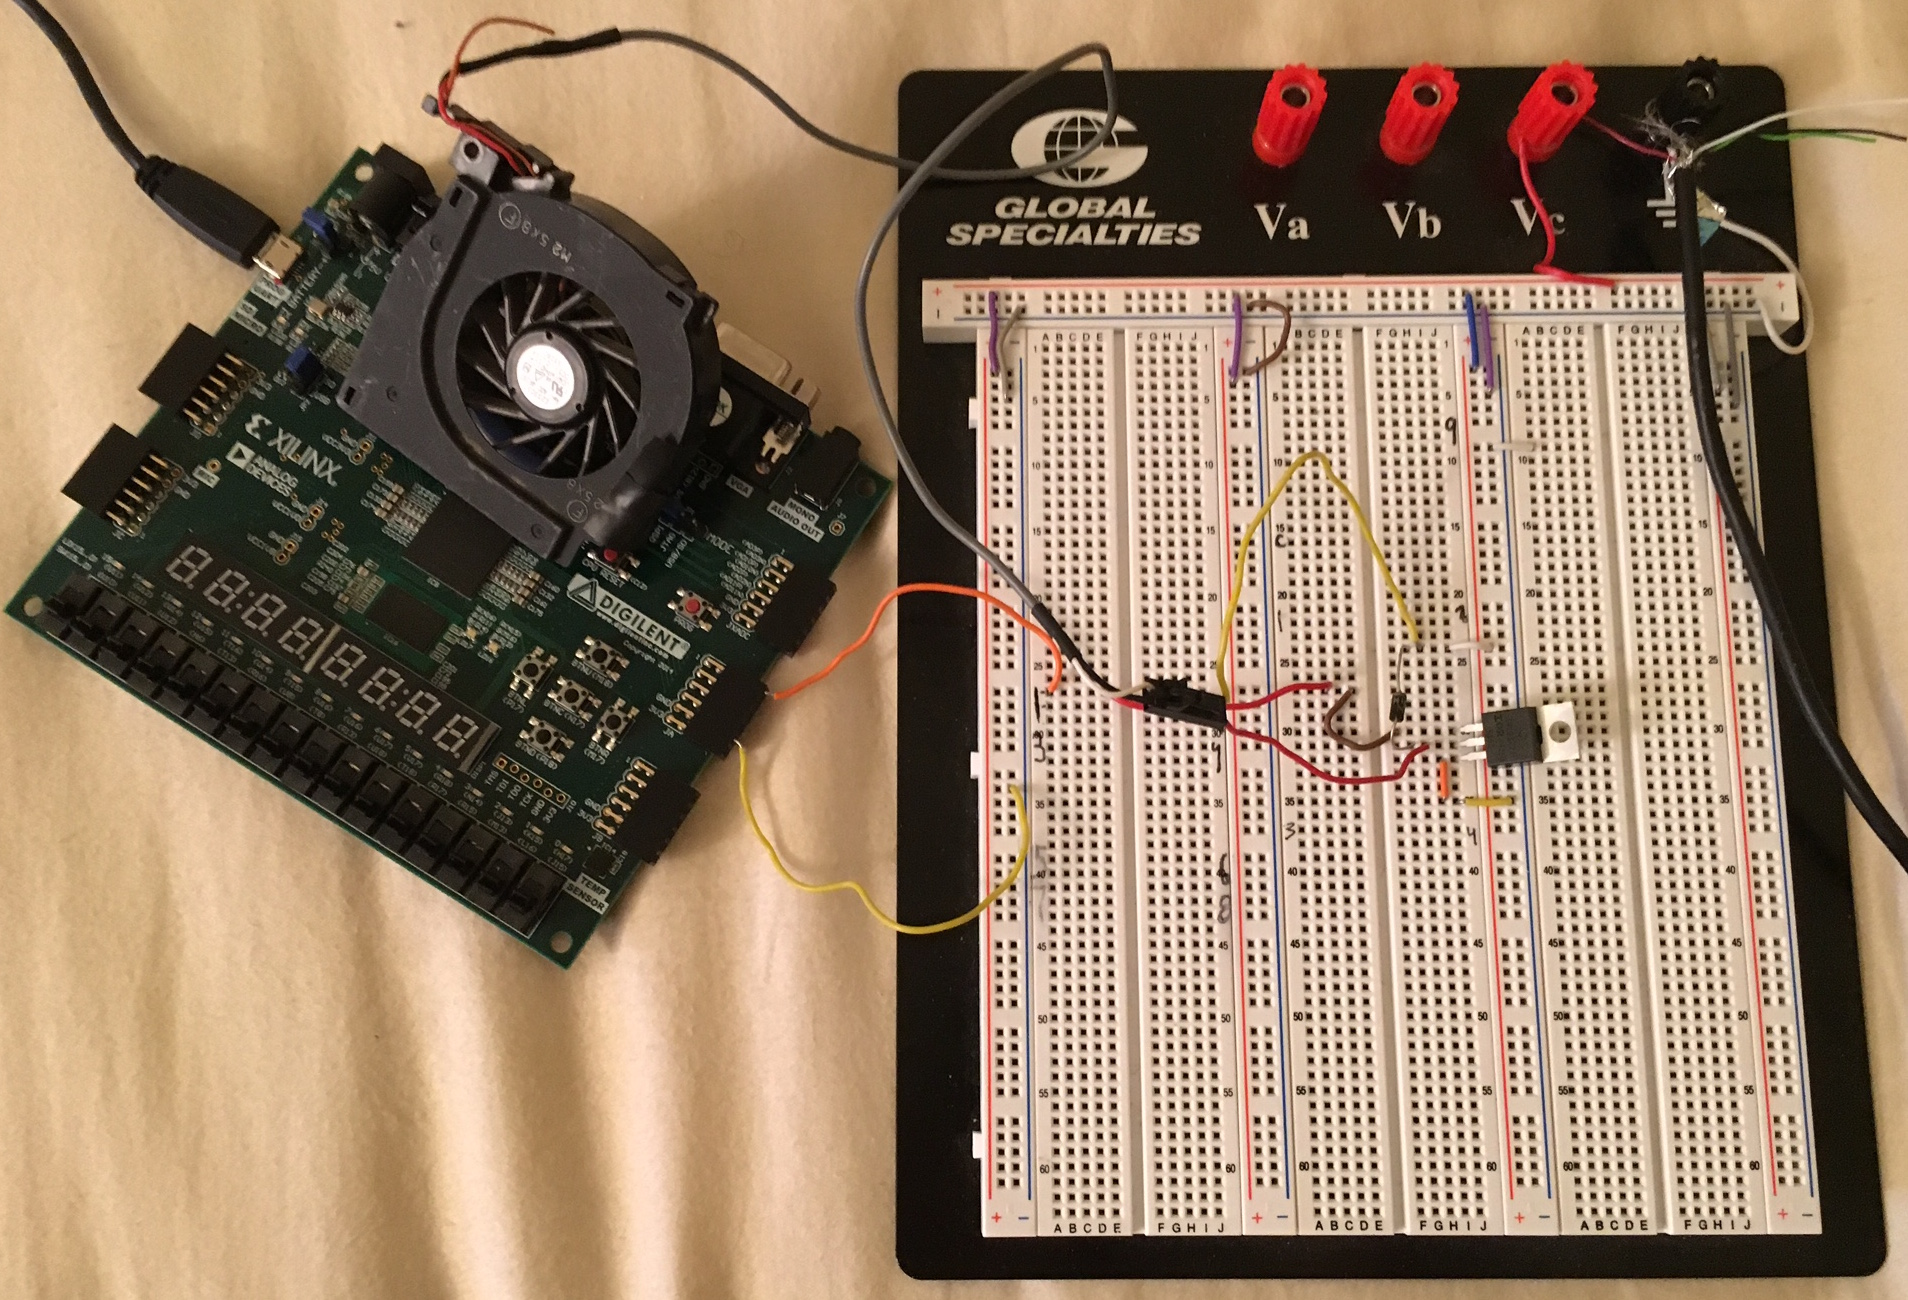
\includegraphics[scale=.2]{images/hardware}\\
\textbf{IMG 1.} Photo of the FPGA with the DC fan and motor driver circuit.\\
\end{center}
\begin{center}
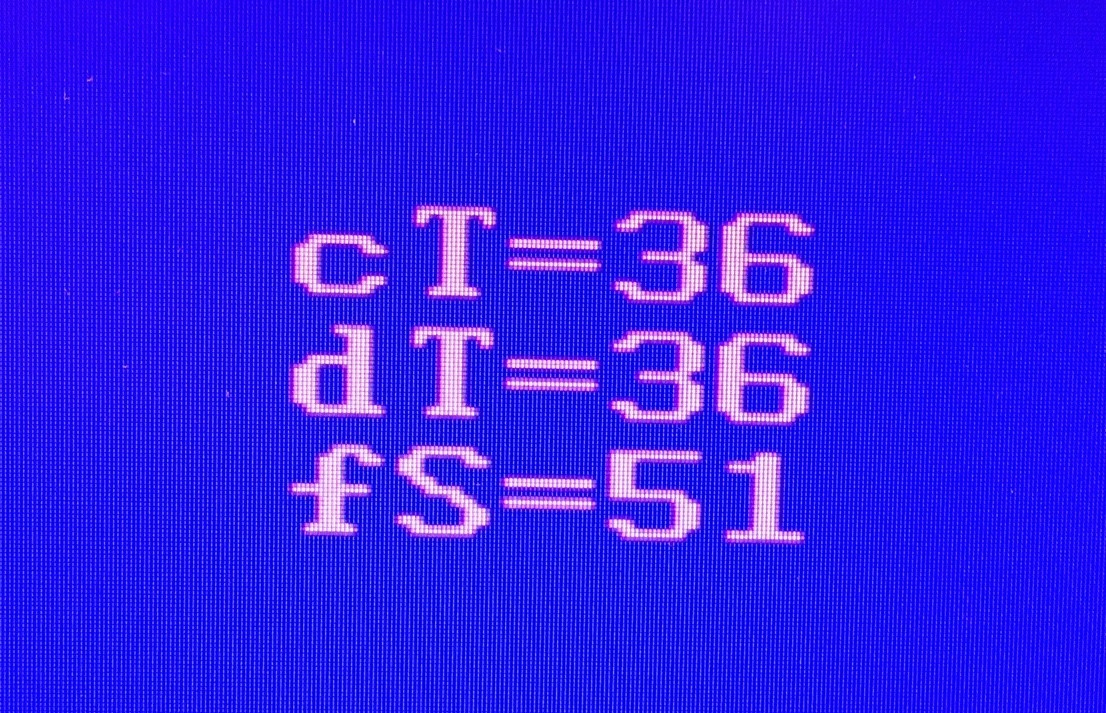
\includegraphics[scale=.2]{images/vgaScreen}\\
\textbf{IMG 2.} Photo of the VGA display during operation.\\
\end{center}

\newpage
\section{References}
[1] \url{http://bytebash.com/2011/10/rs232-uart-vhdl} \newline
[2] \url{http://www.xilinx.com/support/documentation/user_guides/ug480_7Series_XADC.pdf}, page 23 \newline
[3] \url{https://www.adafruit.com/products/355} \newline
[4] Special thanks to Andrew Budd for lending me his fan.\newline
[5] Thanks Dr. Chandy for providing the VGA, BRAM and Char8x1LUT modules.\newline
[6] \url{http://www.mathworks.com/products/sysid/}\newline
[7] \url{http://www.mathworks.com/discovery/pid-tuning.html}
\section{Appendix}
1. VHDL implementation of main components.
\end{document}


